\section{Phương pháp thực nghiệm khoa học}

\

Để tìm ra những kết quả khoa học, chúng ta cần sử dụng \defText{phương pháp thực nghiệm khoa học}. Về mặt bằng chung, phần lớn các phương pháp đó đều phải trải qua những giai đoạn:

\begin{enumerate}[label=\protect\textbf{\color{colorEmphasis}\arabic*.}]
    \item \defText{Quan sát}: Nhận ra một hiện tượng lạ hoặc một vấn đề nảy sinh trong tự nhiên.
    \item \defText{Đặt câu hỏi}: Xác định rõ vấn đề: ``Tại sao hiện tượng này xảy ra?'', ``Nó vận hành như thế nào?''.
    \item \defText{Xây dựng giả thuyết}: Đưa ra một câu trả lời tạm thời có tính lô-gích để giải thích hiện tượng. \label{step:hypo}
    \item \defText{Dự đoán}: Suy luận ra các hệ quả nếu giả thuyết đúng: ``Nếu giả thuyết $A$ là đúng, thì khi làm được $X$, kết quả phải là $Y$''.
    \item \defText{Thực nghiệm}: Tiến hành thí nghiệm để thu thập dữ liệu, các khẳng định, các sự thật. Đây là bước đối chiếu dự đoán với thực tế.
    \item \defText{Phân tích kết quả}: Sử dụng toán học và lập luận lô-gích để xử lí dữ liệu thu được và qua đó kiểm tra kết quả thực tế có khớp với dự đoán không.
    \item \defText{Kết luận và Điều chỉnh}:
          \begin{itemize}
              \item Nếu kết quả khớp: Giả thuyết được tạm chấp nhận.
              \item Nếu kết quả sai: Giả thuyết bị bác bỏ, ta phải quay lại bước \ref{step:hypo} để xây dựng giả thuyết mới.
          \end{itemize}
\end{enumerate}

\begin{figure}[H]
    \centering
    \begin{tikzpicture}[
            node distance=0.8cm and 2cm,
            box/.style={rectangle, draw=colorEmphasisCyan, thick, fill=colorEmphasisCyan!10, minimum width=6cm, minimum height=1cm, align=center, rounded corners=3pt},
            decision/.style={diamond, aspect=2.5, draw=colorEmphasis, thick, fill=colorEmphasis!10, minimum width=3cm, minimum height=1cm, align=center},
            arrow/.style={->, >=stealth, thick, draw=black}
        ]
        % Nodes
        \node[box] (step1) {\textbf{1. Quan sát}};
        \node[box, below=of step1] (step2) {\textbf{2. Đặt câu hỏi}};
        \node[box, below=of step2] (step3) {\textbf{3. Xây dựng giả thuyết}};
        \node[box, below=of step3] (step4) {\textbf{4. Dự đoán}};
        \node[box, below=of step4] (step5) {\textbf{5. Thực nghiệm}};
        \node[box, below=of step5] (step6) {\textbf{6. Phân tích kết quả}};
        \node[decision, below=1cm of step6] (step7) {\textbf{7. Kết quả}\\\textbf{có khớp không?}};
        \node[box, draw=colorEmphasisGreen, fill=colorEmphasisGreen!10, below=1cm of step7] (accept) {\textbf{Chấp nhận giả thuyết}};

        % Arrows
        \draw[arrow] (step1) -- (step2);
        \draw[arrow] (step2) -- (step3);
        \draw[arrow] (step3) -- (step4);
        \draw[arrow] (step4) -- (step5);
        \draw[arrow] (step5) -- (step6);
        \draw[arrow] (step6) -- (step7);
        \draw[arrow] (step7) -- node[right, font=\bfseries] {Có} (accept);

        % Feedback loop
        \draw[arrow] (step7.west) -- node[above, font=\bfseries] {Không (Bác bỏ)} ++(-3.5,0) |- (step3.west);
        \draw[arrow] (accept.east) -- ++(1.5,0) |- (step1.east);
    \end{tikzpicture}
    \caption{Sơ đồ khối phương pháp thực nghiệm khoa học}
\end{figure}

Cần lưu ý rằng quá trình nghiên cứu và thực nghiệm khoa học có tính luân hồi. Các nhà khoa học không chỉ dừng lại ở một kết quả, mà họ tìm cách tiếp tục mở rộng và hoàn thiện nó, làm cho nền khoa học ngày càng được hệ thống hóa và chính xác hơn. Quá trình này có thể diễn ra xuyên suốt nhiều năm, tậm chí nhiều thế hệ.

Tuy rằng phương pháp tác giả vừa mô tả là vô cùng phổ biến, không phải lúc nào một phát hiện khoa học đều đi qua đầy đủ các bước này. Một số lượng lớn những kết quả đi đến từ việc thử sai hàng loạt kết hợp với phát hiện ngẫu nhiên. Xpen-xơ Xin-vơ\footnote{Spencer Silver (1941 -- 2021).}, trong quá trình nghiên cứu chất siêu dính cho ngành hàng không, đã vô tình tạo ra những ``vi cầu'' có độ dính cực thấp. Trong một thời gian dài, không ai để ý đến phát hiện này, cho đến khi Ạt-Phrai\footnote{Art Fry (Năm sinh 1931).}, một đồng nghiệp của Xpen-xơ, đã cảm thấy vô cùng phiền phức vì những mảnh giấy đánh dấu trang nhạc cứ rơi ra ngoài trong một buổi tập hát của nhà thờ. Ông nhớ lại loại keo ``thất bại'' của Xpen-xơ và nhận ra đó chính là thứ mình cần: một loại dấu trang dính được nhưng bóc ra dễ dàng mà không làm hỏng giấy. Thế là những mẩu giấy ghi chú như ở hình \ref{fig:post_it} được ra đời. 

\begin{figure}[h]
    \centering
    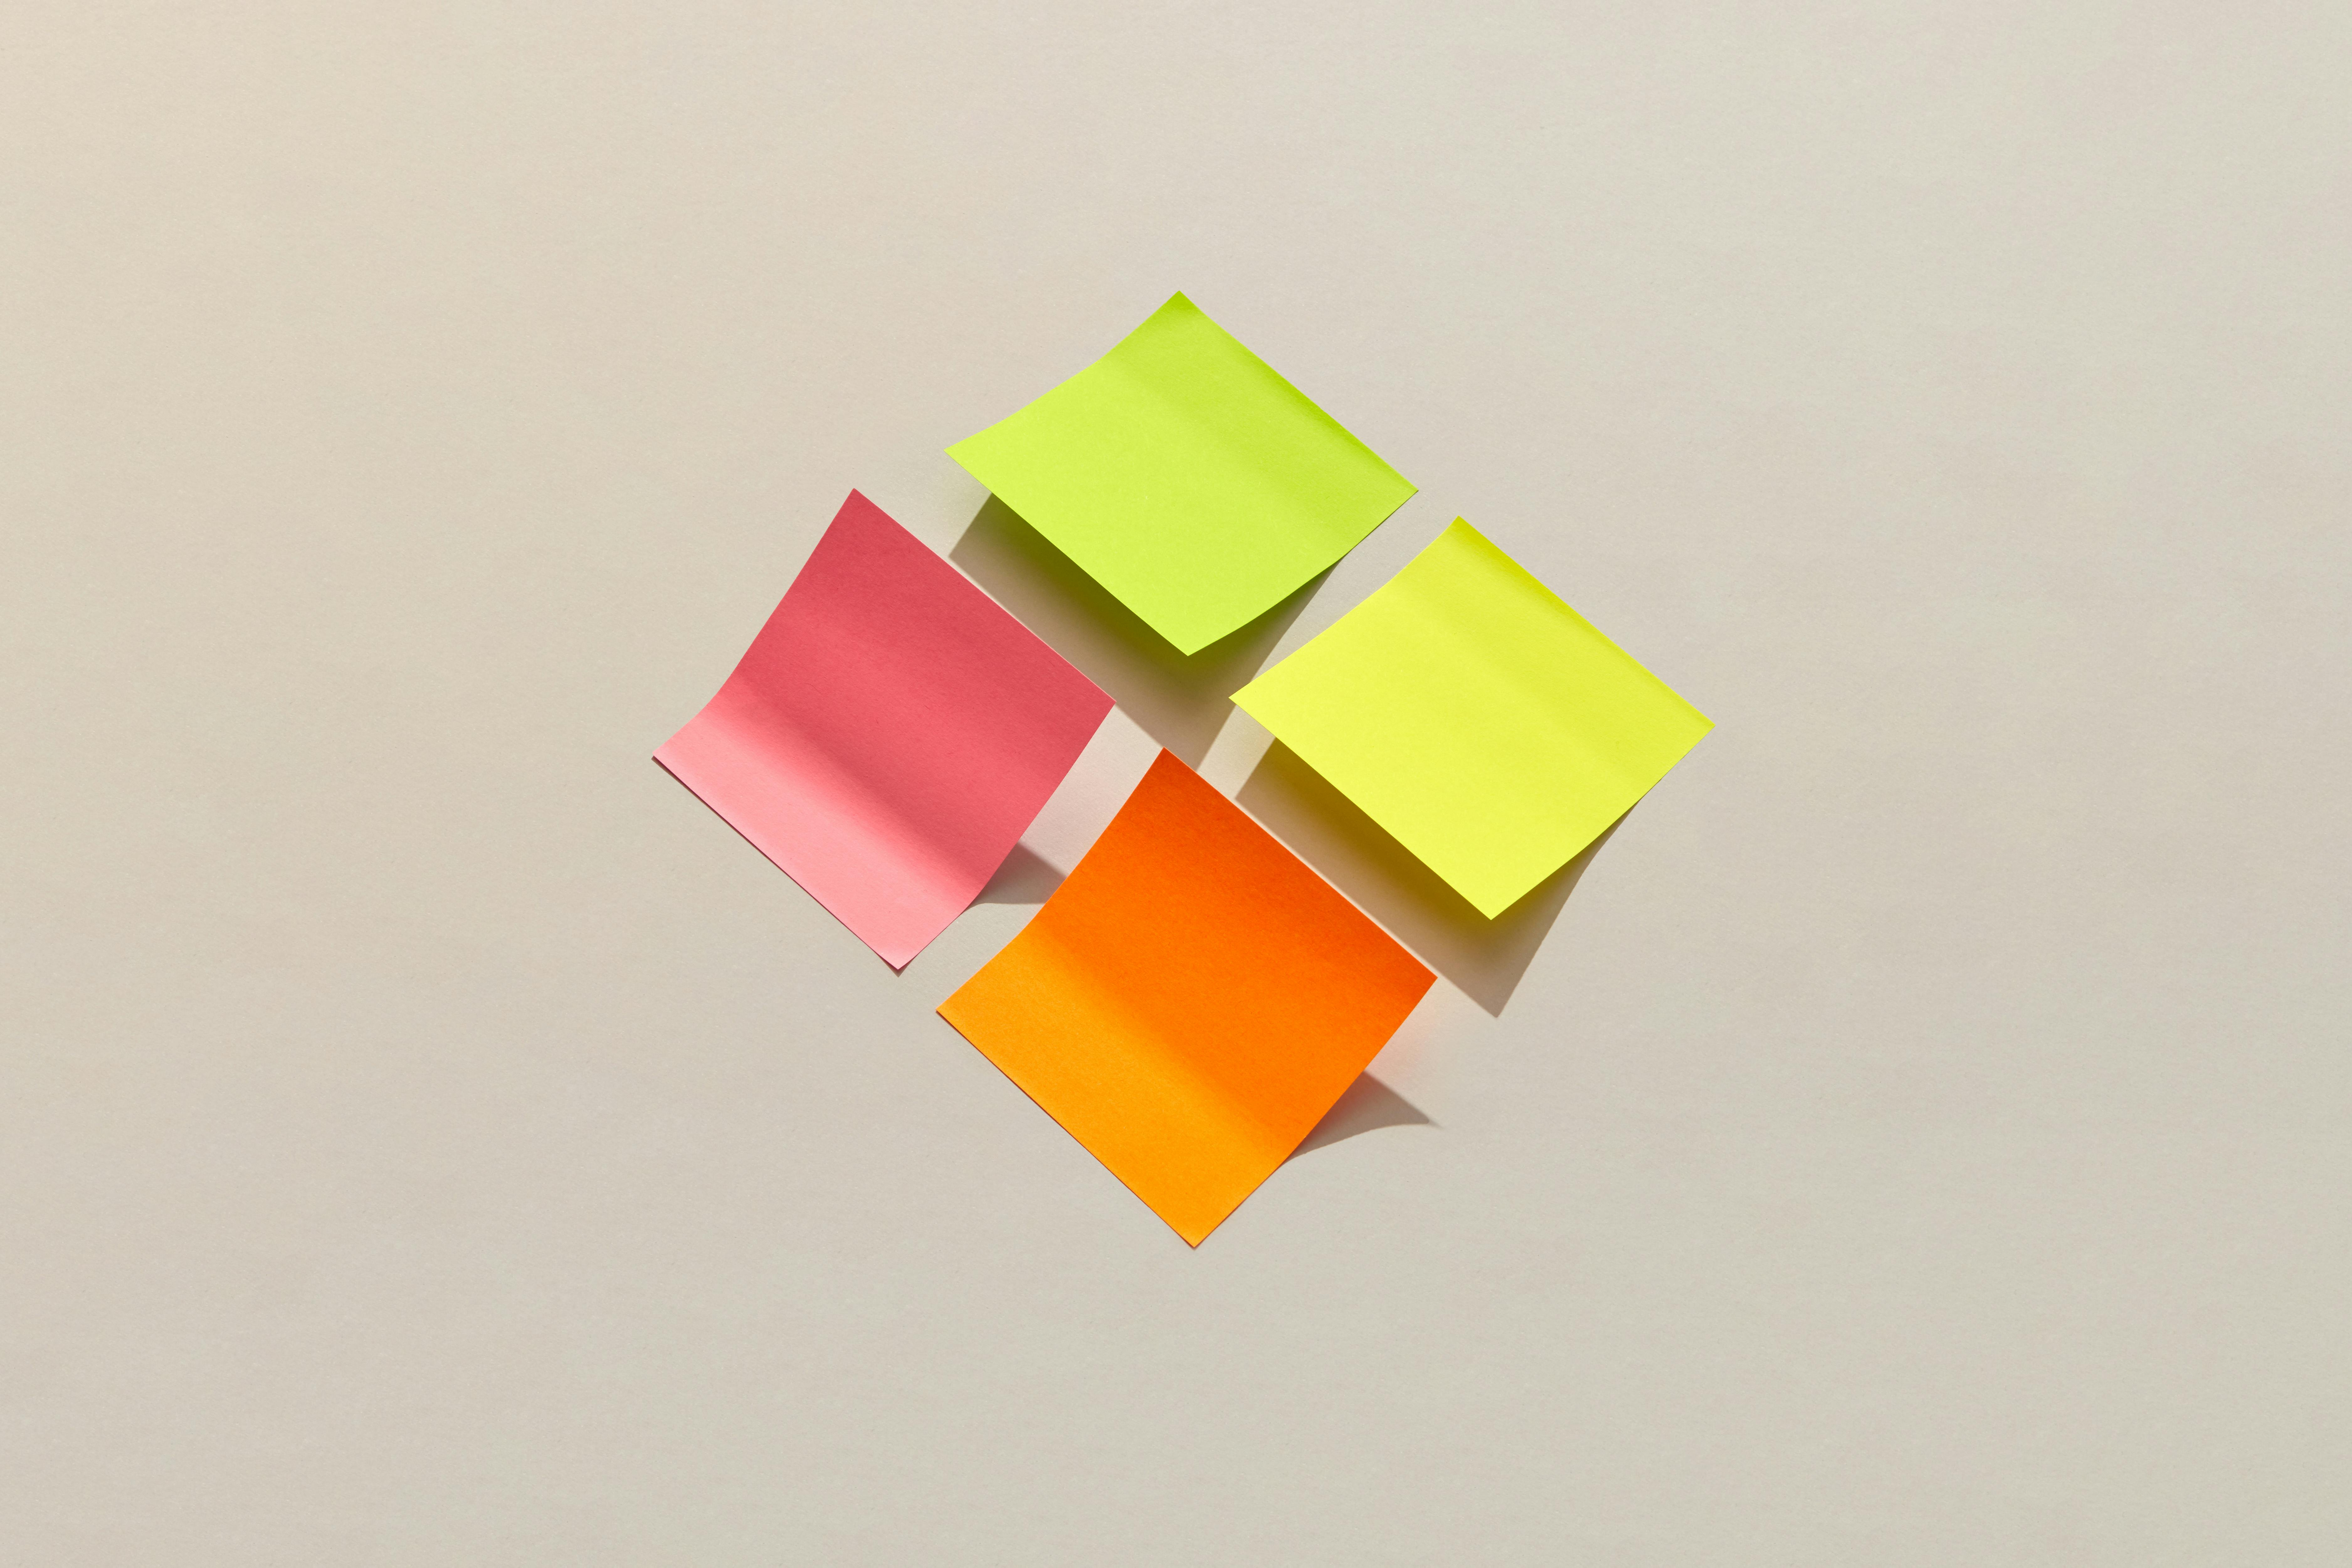
\includegraphics[width=0.6\textwidth]{images/post_it.jpg}
    \caption{Bốn mẩu giấy ghi chú với màu sắc khác nhau\\
        Nguồn: https://www.pexels.com/photo/photo-of-four-colorful-sticky-notes-6991351/}
    \label{fig:post_it}
\end{figure}

Nhưng nhìn chung, đi theo con đường nào đi chăng nữa, một người học và làm khoa học đều cần phải có những phẩm chất cơ bản: sự tìm tòi, tính chính trực, sự kiên trì, và quan trọng nhất, tính khiêm nhường --- gộp chung, khả năng chấp nhận sai sót của bản thân và chấp nhận những kết luận mới, kể cả khi nó trái với tư duy đang sẵn có. 